\documentclass{beamer}
\usepackage[orientation=portrait, size=a0, scale=1]{beamerposter}
\usepackage{multicol} % This is so we can have multiple columns of text side-by-side
\usepackage{parskip}
%\usepackage{enumitem}
%\setlist[itemize]{parsep=0pt}
%\setlist[enumerate]{parsep=0pt}
%\parindent=0em

%% Bibliography stuff (biblatex):
\usepackage[
backend=bibtex,
firstinits=true, 
isbn=false, 
url=false,
maxbibnames=3,
doi=false,
clearlang=true,
terseinits=true,
citestyle=numeric,
autolang=hyphen,
clearlang=true
]{biblatex} 

\AtEveryBibitem{%
  \clearlist{language}%
}


\renewcommand*{\bibfont}{\small}
\bibliography{library.bib}


\usetheme{BCCRC}
%\usetheme{Madrid}
\setbeamerfont{frametitle}{size={\fontsize{200}{36}}}


\title{Screw: tools for building reproducible \\ single-cell epigenomics workflows}
\author{Kieran O'Neill, Chelsey Fang, Benjamin Decato, Azhar Khandekar, Alexander Goncearenco, Ben Busby, Aly Karsan}
\institute{Genome Sciences Centre, BC Cancer Agency, Vancouver, BC, Canada}


\begin{document}
\begin{frame}[t, squeeze, fragile]
\begin{columns}[t]

%%%%%%%%%%%%%%%%%%%%%%%%%%%%%%%%%%%%%%%%%%%%%%%%%%%%%%%%%%%%%%%%%%%%%%%%%%%%%%%%%%%%
% COLUMN 1
%%%%%%%%%%%%%%%%%%%%%%%%%%%%%%%%%%%%%%%%%%%%%%%%%%%%%%%%%%%%%%%%%%%%%%%%%%%%%%%%%%%%


\begin{column}{.32\textwidth}


\begin{block}{Background: Single-cell DNA Methylation Sequencing}
DNA methylation is a heritable epigenetic mark that shows a strong correlation with transcriptional activity. 
The gold standard for detecting DNA methylation is whole genome bisulfite sequencing (WGBS). 
Recently, WGBS has been performed successfully on single cells (SC-WGBS) \cite{Schwartzman2015}.
The resulting data represents a fundamental shift in the capacity to measure and interpret DNA methylation, especially in rare cell types and contexts where subtle cell-to-cell heterogeneity is crucial, such as in stem cells or cancer. 

\begin{figure}
\begin{center}
\includegraphics[width=0.9\textwidth]{figures/nrg3980-f1.jpg}
\end{center}
\caption[]{\textbf{DNA Methylation, both bulk and single cell}
Schwartzman et al (2015) Nature Reviews in Genetics (used by permission) }
\end{figure}

\end{block}


\begin{block}{Reproducible Research with CWL and Docker}
Reproducible research means completely reproducing a given bioinformatic analysis
This requires having the exact \textbf{data}, \textbf{code} and \textbf{software} that was used.

\begin{itemize}
\item Open data in bioinformatics is a fairly solved problem.
\item Code is getting there with RMarkdown/Jupyter, but could be better.
\item Software versions (and accompanying OS/ecosystem) are a big problem.
\end{itemize}
CWL aims to provide a uniform and fully reproducible way of representing bioinformatics workflows. Docker aims to provide the exact environment in which an analysis was run. Together, they promise to help bioinformaticians to publish fully reproducible research.

As a side effect, Dockstore enables easy sharing of workflow components to help build new workflows. 
\begin{figure}
\begin{center}
\includegraphics[width=0.9\textwidth]{figures/dockstore_logos.png}
\end{center}
\caption{\textbf{Docker, CWL and Dockstore.} CWL workflows (and Docker build files) are kept on GitHub. Quay.io automatically builds Docker images from these. Dockstore enables sharing of CWL-specified tools and workflows, along with a Docker image containing exact software.}
\end{figure}
\end{block}


\begin{block}{Screw: Single Cell Reproducible Epigenomics Workflow}
%\includegraphics[width=0.2\textwidth]{figures/screw_logo_1600.png}
Screw aims to provide a series of CWL+Dockerised mini-workflows and workflow components for creating fully reproducible single-cell DNA methylation analyses.

\end{block}


\begin{block}{What SC-WGBS Data Looks Like}
Lots of cells, but lots of dropout too.

\begin{figure}
\begin{center}
\includegraphics[width=0.9\textwidth]{figures/hoxa9_meth.png}

\end{center}
\caption{\textbf{DNA methylation around the \textit{HOXA9} TSS, from 100 single cells.}  Blue blocks indicate methylated CpGs, white unmethylated. Teal indicates missing data. DNA methylation data is very sparse -- only a handful of libraries have any coverage at all within a given window. Data from \cite{Farlik2016}; BigWIGS generated by Screw.}
\end{figure}
\end{block}




\end{column}

%%%%%%%%%%%%%%%%%%%%%%%%%%%%%%%%%%%%%%%%%%%%%%%%%%%%%%%%%%%%%%%%%%%%%%%%%%%%%%%%%%%%
% COLUMN 2
%%%%%%%%%%%%%%%%%%%%%%%%%%%%%%%%%%%%%%%%%%%%%%%%%%%%%%%%%%%%%%%%%%%%%%%%%%%%%%%%%%%%

\begin{column}{.65\textwidth}
\vspace*{-\baselineskip}
  \begin{columns}[t,totalwidth=\textwidth]
    \begin{column}{.48\textwidth}
	%Second column, above figure
    
	
	\end{column}

	\begin{column}{.48\textwidth}
	%Third column, above figure
	
	\end{column}
  \end{columns}

	\begin{block}{Screw Workflow}
	\begin{figure}
	\begin{center}
  \includegraphics[width=0.95\textwidth]{figures/workflow_diagram.pdf}
  \end{center} 
  \caption{\textbf{The Screw workflow, showing completed and short-term planned functionality.} }
  \end{figure}
  \end{block}
  \begin{columns}[t,totalwidth=\textwidth]


\begin{column}{.48\textwidth}
   

% Second column, below figure   
\begin{block}{Preprocessing: Format Interconversion}
	One of the challenges in DNA methylation is the lack of a standard data format. BED files are poorly suited, since multiple data columns are needed. Also, CpG sites are all point locations, so the end column is unncessary. WIG/BigWIG can help, but don't support enough data columns. The consequence is that every data set has its own custom BED-like format. We are working on providing 
\begin{figure}
\begin{center}
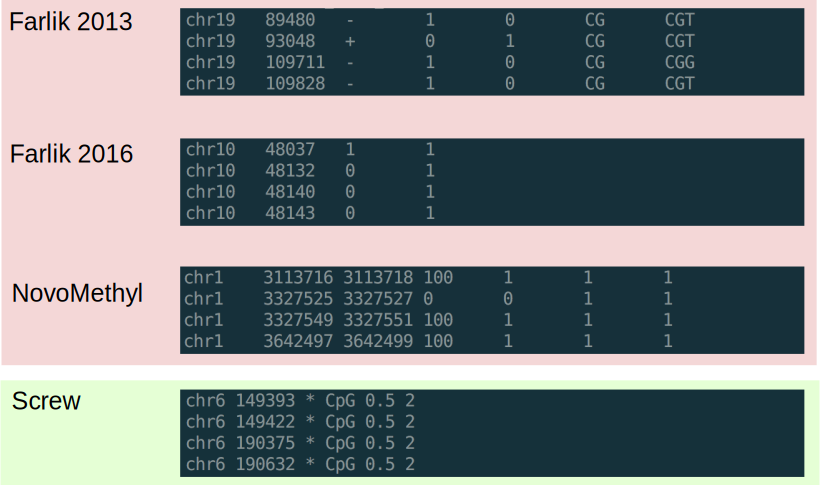
\includegraphics[width=0.9\textwidth]{figures/data_types.pdf}
\caption{\textit{Diverse DNA methylation formats.} Formats from two published papers (\cite{Farlik2013} and \cite{Farlik2016}), NovoMethyl output format (unpublished), and Screw's standard internal format.}
\end{center}
\end{figure}

\end{block}

\begin{block}{Clustering}
\begin{figure}
\begin{center}
\includegraphics[width=0.8\textwidth]{figures/farlik_heatmap.pdf}
\caption{\textbf{Clustering of data from \cite{Farlik2016}.} The data was subset to only include enhancer sites from Enhancer Atlas found in CD34+ bone marrow cells. Only 47/100 cells had coverage in those regions.}
\end{center}
\end{figure}


\end{block}


\end{column}

	\begin{column}{.48\textwidth}
% Third column, below figure   

\begin{block}{CWL+Docker Stumbling Blocks}
\begin{itemize}
\item CWL does not have a good way of processing a whole directory full of files, then passing them on to a single tool.
\item Quay.io maps tags to GitHub branches, but Docker treats tags like Git graph nodes, leading to problems refreshing branches while developing.
\item Our hyper-secure clinical IT environment won't let us use Docker, but will install Udocker, which CWL runner does not support (yet?)
\end{itemize}
\end{block}



\begin{block}{Future Plans}
Many methods are currently being developed, and some have debuted in papers without (yet) an accompanying methods paper. In future we plan to include functionality for:
\begin{itemize}
\item tSNE plotting
\item Epiphylogenomics
\item DeepCpG
\item Other machine learning pipelines (e.g. from \cite{Farlik2016}) 
\end{itemize}

\end{block}


\begin{block}{Powered by hackathons and interns}
Screw was initially created during the NCBI Genomics Hackathon in March 2017, organised by Ben Busby. Ben organises awesome hackathons that drive a lot of new open source tool development. Since then, Chelsey Fang, a summer intern, has been working on the framework.


\begin{figure}
\begin{center}
  \includegraphics[width=0.7\textwidth]{figures/hackathon_team.jpg}
  \includegraphics[width=0.2\textwidth]{figures/chelsey.jpg}
\end{center}
\caption{\textbf{The Screw team.} From left to right, Azhar Khandekar, Benjamin Decato, , Kieran O'Neill, Alexander Goncearenco; separate photo: Chelsey Fang.}
\end{figure}

\end{block}

\begin{block}{References}

\printbibliography[heading=none]
\end{block}



\begin{block}{Contact/GitHub}
\textbf{Code/examples:} \verb1https://github.com/Epigenomics-Screw1  

\textbf{Kieran O'Neill:} koneill@bcgsc.ca 

\end{block}
 
\end{column}

  \end{columns}
\end{column}


\end{columns}

\end{frame}

\end{document}
